\documentclass[border=3mm,tikz,preview]{standalone}
\usepackage[utf8]{inputenc}
\usepackage{amsmath,amssymb,amsfonts}
\usepackage{graphicx}
\usepackage{tikz}
\usetikzlibrary{shapes.geometric, arrows.meta, positioning, shadows, calc, fit, backgrounds}
\usepackage{xcolor}
\begin{document}

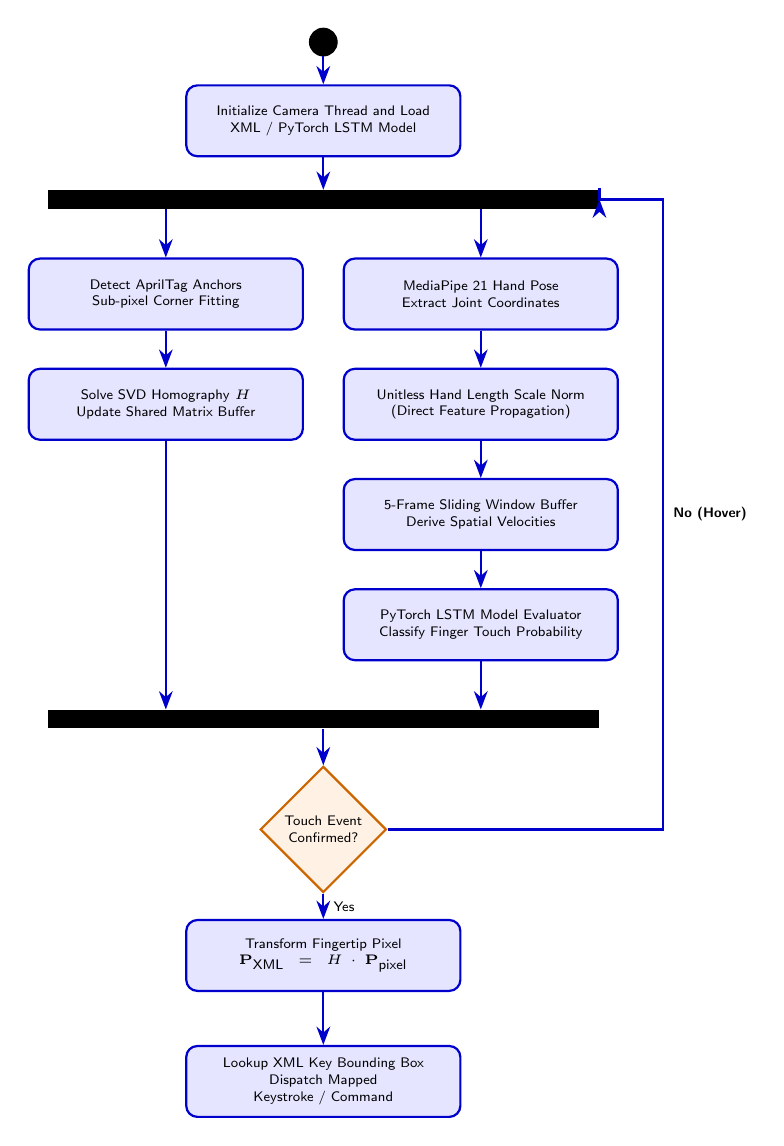
\begin{tikzpicture}[
    start/.style = {circle, draw=black, fill=black, inner sep=0pt, minimum size=10pt},
    stop/.style = {circle, draw=black, fill=white, inner sep=0pt, minimum size=12pt},
    activity/.style = {rectangle, draw=blue!80!black, fill=blue!10!white, thick, rounded corners=4pt, align=center, font=\sffamily\tiny, minimum height=0.9cm, text width=3.2cm, inner sep=4pt},
    decision/.style = {diamond, draw=orange!80!black, fill=orange!10!white, thick, align=center, font=\sffamily\tiny, inner sep=2pt},
    arrow/.style = {draw=blue!80!black, ->, >=Stealth, thick}
]

\node (st) [start] at (0,0) {};
\node (a_init) [activity] at (0, -1.0) {Initialize Camera Thread and Load XML / PyTorch LSTM Model};

% Fork Bar
\node (fork) [rectangle, fill=black, minimum height=3pt, minimum width=7cm] at (0, -2.0) {};

% Left Branch: AprilTag
\node (a_tag) [activity] at (-2.0, -3.2) {Detect AprilTag Anchors\\Sub-pixel Corner Fitting};
\node (a_homog) [activity] at (-2.0, -4.6) {Solve SVD Homography $H$\\Update Shared Matrix Buffer};

% Right Branch: MediaPipe Pose
\node (a_pose) [activity] at (2.0, -3.2) {MediaPipe 21 Hand Pose\\Extract Joint Coordinates};
\node (a_norm) [activity] at (2.0, -4.6) {Unitless Hand Length Scale Norm\\(Direct Feature Propagation)};
\node (a_window) [activity] at (2.0, -6.0) {5-Frame Sliding Window Buffer\\Derive Spatial Velocities};
\node (a_lstm) [activity] at (2.0, -7.4) {PyTorch LSTM Model Evaluator\\Classify Finger Touch Probability};

% Join Bar
\node (join) [rectangle, fill=black, minimum height=3pt, minimum width=7cm] at (0, -8.6) {};

\node (d_touch) [decision] at (0, -10.0) {Touch Event\\Confirmed?};
\node (a_map) [activity] at (0, -11.6) {Transform Fingertip Pixel\\$\mathbf{P}_{\text{XML}} = H \cdot \mathbf{P}_{\text{pixel}}$};
\node (a_exec) [activity] at (0, -13.2) {Lookup XML Key Bounding Box\\Dispatch Mapped Keystroke / Command};

\draw [arrow] (st) -- (a_init);
\draw [arrow] (a_init) -- (fork);

\draw [arrow] (fork.south -| a_tag.north) -- (a_tag);
\draw [arrow] (a_tag) -- (a_homog);
\draw [arrow] (a_homog) -- (join.north -| a_homog.south);

\draw [arrow] (fork.south -| a_pose.north) -- (a_pose);
\draw [arrow] (a_pose) -- (a_norm);
\draw [arrow] (a_norm) -- (a_window);
\draw [arrow] (a_window) -- (a_lstm);
\draw [arrow] (a_lstm) -- (join.north -| a_lstm.south);

\draw [arrow] (join) -- (d_touch);
\draw [arrow] (d_touch) -- node[right, font=\sffamily\tiny]{Yes} (a_map);
\draw [arrow] (a_map) -- (a_exec);
\draw [arrow] (d_touch.east) -- ++(3.5,0) -- node[right, font=\sffamily\tiny]{\textbf{No (Hover)}} ++(0, 8.0) -| (fork.east);

\end{tikzpicture}

\end{document}
